\documentclass[a4paper]{article}
\usepackage[utf8]{inputenc}
\usepackage[T1]{fontenc}
\usepackage[intlimits]{amsmath}
\usepackage{amsfonts}
\usepackage{amssymb}
\usepackage[export]{adjustbox}
\usepackage{graphicx}
\setlength{\parindent}{0pt}
\usepackage[left=1in, right=1in, top=1in, bottom=1in]{geometry}
\usepackage{float}
\usepackage{multicol}
\usepackage{listings}
\usepackage{xcolor}
\usepackage{cancel}
\usepackage{bm}
\usepackage{hyperref}
\setcounter{tocdepth}{1}
\usepackage[titletoc]{appendix}
\hypersetup{
	colorlinks=true,
	linkcolor=blue,
	filecolor=blue,
	urlcolor=blue,
}

\newcommand\blfootnote[1]{%
	\begingroup
	\renewcommand\thefootnote{}\footnote{#1}%
	\addtocounter{footnote}{-1}%
	\endgroup
}

\begin{document}
	
	\Huge\textbf{Chain Belt C-C Distance Calculator}
	\newline
	\LARGE AMB Calculator
	
	\vspace{0.5cm}
	\normalsize
	
	This calculator determines the proper center-to-center spacing between two sprockets or pulleys, as based on the belt/chain length or an approximate center-to-center distance.\\
	
	The calculator comes loaded with the standard types of belt and chain used in FRC, and their respective pitch lengths, $ p $. If you want a non-standard pitch length, you can set that by choosing a "Custom" type. For the standard types, useful dimensions are also shown including the width, thickness, and weight. These dimensions do not affect the calculations. Suggested adders (i.e. the recommended amount to over/under tension the system) and load ratings are given for some types, though these values may vary based on the source of the belt/chain and team preference.\\
	
	For this document we will use the nomenclature for chain, though the equations apply identically to belts.\\
	
	To calculate the pitch diameter of each sprocket with $ n $ teeth, we use the formula:
	
	\begin{equation}
		d_p = \frac{n \cdot p}{\pi}
	\end{equation}\\
	
	Halving this value gives us the pitch radius for each sprocket, $ r_x = \frac{n_x p}{2\pi} $.\\
	
	Defining the total chain length as $ L $ and the number of links as $ \ell $, we know $ L = \ell \cdot p $. We can also find the total chain length geometrically using the sprocket radii and center-to-center distance $ D $.
	
	\begin{figure}[H]
		\centering
		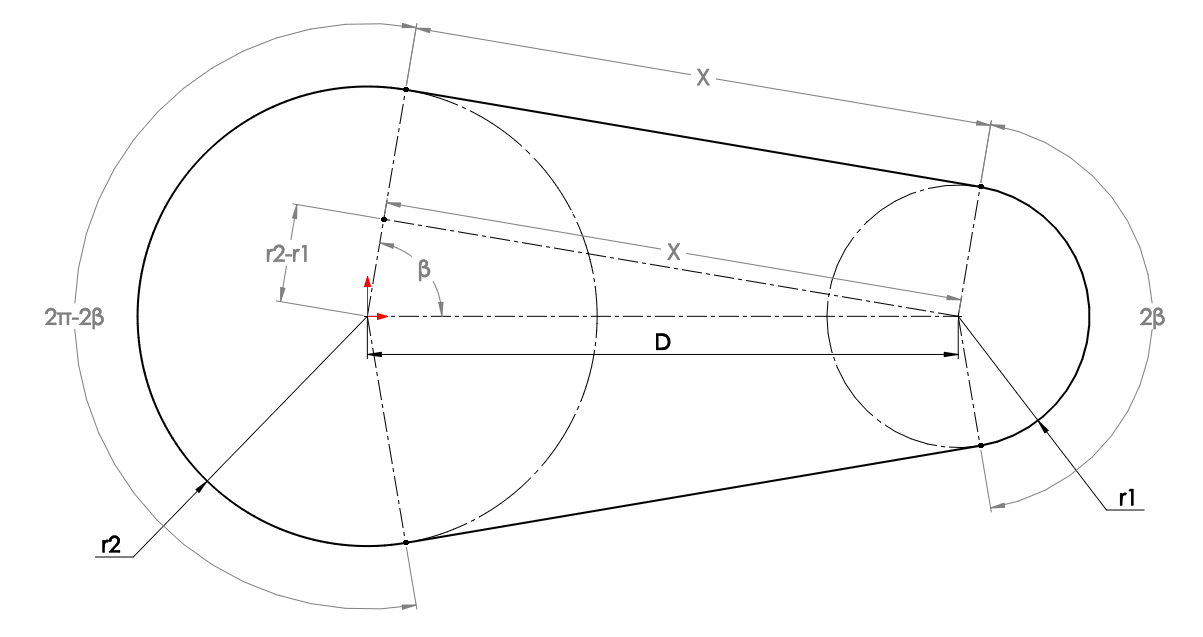
\includegraphics[width=0.9\linewidth]{../img/equations_chain}
	\end{figure}

	Adding up the various sections of the chain path, it is clear that:
	
	\begin{equation} \label{Lbase}
		L = 2X + r_1 \cdot 2\beta + r_2 \cdot \left( 2\pi - 2\beta \right)
	\end{equation}\\
	
	Using the Pythagorean theorem and trigonometry on the right triangle in the center of the diagram, we can see that:
	
	\begin{equation} \label{X}
		D^2 = X^2 + \left( r_2 - r_1 \right)^2 \implies X = \sqrt{D^2 - \left( r_1 - r_2 \right)^2}
	\end{equation}
	
	\begin{equation} \label{beta}
		\beta = \cos^{-1} \left( \frac{r_2 - r_1}{D} \right) = \cos^{-1} \left( \frac{r_1 - r_2}{D} \right)
	\end{equation}\\
	
	Substituting (\ref{X}) and (\ref{beta}) into (\ref{Lbase}) gives:
	
	\begin{gather} \label{L}
	\begin{aligned}
		L &= 2 \sqrt{D^2 - (r_1 - r_2)^2} + r_1 \cdot 2 \cos^{-1} \left( \frac{r_1 - r_2}{D} \right) + r_2 \cdot \left( 2\pi - 2\cos^{-1} \left( \frac{r_1 - r_2}{D} \right) \right) \\
		&= 2 \sqrt{D^2 - \left( r_1 - r_2 \right)^2} + 2 \left( r_1 - r_2 \right) \cos^{-1} \left( \frac{r_1 - r_2}{D} \right) + 2\pi r_2
	\end{aligned}
	\end{gather}\\
	
	Unfortunately, this equation cannot be solved analytically for $ D $. So instead, the calculator solves it numerically using the \href{https://en.wikipedia.org/wiki/Newton\%27s_method}{Newton-Raphson Method}. For the calculation based on number of links, our goal is $ L = \ell \cdot p $ and our initial guess is $ D = \frac{1}{2} L $, which would be the case if both sprockets had zero pitch diameter. For the approximate center-to-center distance calculation, our initial guess for $ D $ is the approximate distance. To get the target value, we plug in the approximate distance to (\ref{L}) and find the non-integer number of links that would produce. That number is then rounded to an even multiple in the direction specified to get $ \ell $, and the target is $ L = \ell \cdot p $. The numerical solver continues until a precision of at least $ 10^{-3} $ is reached.
	
	\blfootnote{The derivation of this algorithm is based on work done by Clem McKown of FRC team 1640.}
	
	
\end{document}